\documentclass{beamer}
\usepackage[utf8]{inputenc}
\usetheme{Madrid}
\usepackage{amssymb}
\usepackage{pifont}
\usepackage{xcolor}
\usepackage{bigints}
\usepackage{mathrsfs}
\definecolor{dgreen}{rgb}{0.,0.6,0.}
\newcommand{\cmark}{{\color{dgreen}\ding{51}}}%
\newcommand{\xmark}{{\color{red}\ding{55}}}%
\newcommand{\bmark}{{\color{orange}$\sim$}}%

\usepackage{amsmath}
\usepackage{cancel}
\DeclareMathOperator*{\argmax}{argmax}
\DeclareMathOperator*{\argmin}{argmin}

\beamertemplatenavigationsymbolsempty
%for backup slides
\newcommand{\backupbegin}{
   \newcounter{finalframe}
   \setcounter{finalframe}{\value{framenumber}}
}
\newcommand{\backupend}{
   \setcounter{framenumber}{\value{finalframe}}
}


\AtBeginSection[
  {\frame<beamer>{\frametitle{Table des matières}   
    \tableofcontents[currentsection,currentsection]}}%
]%
{
  \frame<beamer>{ 
    \frametitle{Table des matières}   
    \tableofcontents[currentsection,currentsection]}
}


\title[Présentation CSI]{Présentation CSI\\ Étude de Vlasov-Poisson 1D$x$-1D$v$}
\subtitle{Optimisation de WENO pour Vlasov-Poisson}
\author{Josselin Massot}
\institute{IRMAR}
\date{24 avril 2019}

\defbeamertemplate*{title page}{customized}[1][]
{
  \vfill
  {\usebeamerfont{title}\inserttitle}\par
  {\usebeamerfont{subtitle}\usebeamercolor[bg]{subtitle}\insertsubtitle}\par
  \bigskip
  \vfill
  \hfill\usebeamerfont{author}\insertauthor\par\par
  \hfill\textcolor{black}{Encadré par~: Anaïs Crestetto\\\hfill et Nicolas Crouseilles}\par
  \vfill
  \hfill\usebeamerfont{date}\insertdate
}

\begin{document}

\begin{frame}[plain,t]
  \titlepage
\end{frame}

\begin{frame}{Table des matières}
  \tableofcontents
\end{frame}

\section{Introduction - Vlasov-Poisson et WENO}
\begin{frame}{Vlasov-Poisson}
  $$
    \begin{cases}
      \partial_t f + v\partial_x f + E\partial_v f = 0 \\
      \partial_x E = \int_{\mathbb{R}} f\,\mathrm{d}v - 1
    \end{cases}
  $$

  \begin{itemize}
    \item Filamentation dans la solution
      \begin{itemize}
        \item Ordre élevé dans l'espace des phases $(x,v)$
      \end{itemize}
    \item Approche classique : méthode de \emph{splitting} de Strang
      \begin{itemize}
        \item \textbf{Problèmes :} ordre élevé en temps, passage à Vlasov-Maxwell (\emph{splitting} du champ magnétique $B$)
      \end{itemize}
  \end{itemize}
\end{frame}

\begin{frame}{Résumé du stage}
  \textbf{WENO c'est bien !} \cmark

  \ 

  \textbf{MAIS : } instable avec méthode d'Euler explicite en temps (\emph{toy model} pour démonstration, ou simulation test)
  \begin{itemize}
    \item {[R. Wang \& R. J. Spiteri (2007)]} besoin d'au moins \emph{"RK3"} (démonstration faite avec $WENO^{\ell}$)
    \item {[M. Motamed \& C. B. Macdonald \& S. J. Ruuth (2010)]} estimation d'une CFL de $RK(3,3)-WENO^{\ell}$
  \end{itemize}
\end{frame}

\begin{frame}{WENO}
  \textbf{W}eighted \textbf{E}ssentially \textbf{N}on-\textbf{O}scillatory : schéma \emph{DF} non linéaire

  3 estimations sur 3 \emph{stencils} différents, pondérées (poids non linéaires)

  \begin{center}
    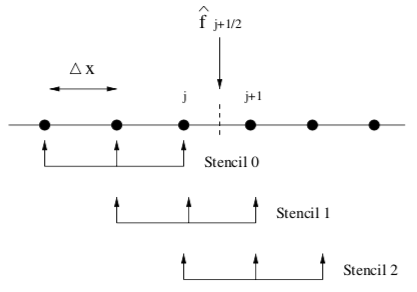
\includegraphics[width=0.5\textwidth]{stencils.png}
  \end{center}

  3 étapes de calcul : \begin{itemize}\item Indicateurs de continuité \item Poids \item Flux \end{itemize}
\end{frame}

\begin{frame}{WENO (les indicateurs de continuité)}
  Résolution de : $$
    \partial_t u + \partial_xf(u) = 0
  $$

  \ 

  $$
    f(u) = f^+(u) + f^-(u)\quad,\quad \frac{df^+}{du}\geq 0\ \text{et}\ \frac{df^-}{du}\leq 0
  $$

  \ 

  \textbf{Indicateurs de continuité} \emph{Indicator of smoothness} \textbf{:}
  $$
      \beta_i^\pm  \gets (f^\pm_{[\![j-2,j+3]\!]})\ ,\ i=0,1,2
  $$
  Approximations de dérivées premières et secondes sur les 3 \emph{stencils}.
\end{frame}

\begin{frame}
  $$
    \begin{aligned}
      \beta_0^+ &= \frac{13}{12}\left( f^+_{j-2} - 2f^+_{j-1} + f^+_{j}   \right)^2\!\!\!\!\!\!&+& \frac{1}{4}\left(  f^+_{j-2} - 4f^+_{j-1} + 3f^+_{j}   \right)^2 \\
      \beta_1^+ &= \frac{13}{12}\left( f^+_{j-1} - 2f^+_{j}   + f^+_{j+1} \right)^2\!\!\!\!\!\!&+& \frac{1}{4}\left(  f^+_{j-1}              -  f^+_{j+1} \right)^2 \\
      \beta_2^+ &= \frac{13}{12}\left( f^+_{j}   - 2f^+_{j+1} + f^+_{j+2} \right)^2\!\!\!\!\!\!&+& \frac{1}{4}\left( 3f^+_{j}   - 4f^+_{j+1} +  f^+_{j+2} \right)^2\\
      & & & \\
      \beta_0^- &= \frac{13}{12}\left( f^-_{j+1} - 2f^-_{j+2} + f^-_{j+3} \right)^2\!\!\!\!\!\!&+& \frac{1}{4}\left( 3f^-_{j+1} - 4f^-_{j+2} +  f^-_{j+3} \right)^2 \\
      \beta_1^- &= \frac{13}{12}\left( f^-_{j}   - 2f^-_{j+1} + f^-_{j+2} \right)^2\!\!\!\!\!\!&+& \frac{1}{4}\left(  f^-_{j}                -  f^-_{j+2} \right)^2 \\
      \beta_2^- &= \frac{13}{12}\left( f^-_{j-1} - 2f^-_{j}   + f^-_{j+1} \right)^2\!\!\!\!\!\!&+& \frac{1}{4}\left(  f^-_{j-1} - 4f^-_{j}   + 3f^-_{j+1} \right)^2
    \end{aligned}
  $$
\end{frame}

\begin{frame}{WENO (les poids)}
  \textbf{Poids non normalisés} :
  $$
      \alpha_i^\pm \gets \frac{\gamma_i}{(\epsilon+\beta_i^\pm)^2}\ ,\  \gamma_i \in\mathbb{R}^*_+\,: \sum_k\gamma_k = 1
  $$
  On prend : $\gamma_0 = \frac{1}{10}, \gamma_1=\frac{6}{10}, \gamma_2=\frac{3}{10}$. Paramètre $\epsilon = 10^{-6}$

  \

  Linéarisation (DL) : $\alpha_i^\pm = \gamma_i + \mathcal{O}(\Delta x^2)$

  \ 

  \textbf{Les poids normalisés} :
  $$
      w_i^\pm \gets \frac{\alpha_i^\pm}{\sum_k\alpha_k^\pm}
  $$

\end{frame}

\begin{frame}{WENO (les flux)}

  $$
    \begin{aligned}
      f_{j+\frac{1}{2}}^+ \gets w_0^+ \left( \frac{2}{6}f^+_{j-2} - \frac{7}{6}f^+_{j-1} + \frac{11}{6}f^+_{j}\right)
                              + w_1^+ \left(-\frac{1}{6}f^+_{j-1} + \frac{5}{6}f^+_{j}   +  \frac{2}{6}f^+_{j+1}\right) \\
                              + w_2^+ \left( \frac{2}{6}f^+_{j}   + \frac{5}{6}f^+_{j+1} -  \frac{1}{6}f^+_{j+2}\right)
    \end{aligned}
  $$

  $$
    \begin{aligned}
      f_{j+\frac{1}{2}}^- \gets w_2^- \left(-\frac{1}{6}f^-_{j-1} + \frac{5}{6}f^-_{j}   + \frac{2}{6}f^-_{j+1}\right)
                              + w_1^- \left( \frac{2}{6}f^-_{j}   + \frac{5}{6}f^-_{j+1} - \frac{1}{6}f^-_{j+2}\right) \\
                              + w_0^- \left(\frac{11}{6}f^-_{j+1} - \frac{7}{6}f^-_{j+2} + \frac{2}{6}f^-_{j+3}\right)
    \end{aligned}
  $$

  $$
  \boxed{
    (\partial_x f(u))_j \approx \frac{1}{\Delta x}\left[(f_{j+\frac{1}{2}}^+ - f_{j-\frac{1}{2}}^+) + (f_{j+\frac{1}{2}}^- - f_{j-\frac{1}{2}}^-)\right]
    }
  $$
\end{frame}


\section{Automatisation de calcul de CFL}
\begin{frame}{Outils pour l'estimation de CFL}
  \textbf{Analyse de von Neumann} : permet l'analyse de schémas linéaires $$u_{j+k} \mapsto e^{ik\phi}$$ fonction de $\phi$ : \underline{coefficient d'amplification} du schéma \begin{itemize}
    \item Analyse de schémas non-linéaires possible mais pas systématique
    \item Écriture du schéma sous la forme : $(\partial_x u^n) \approx W(\phi)u^n$
  \end{itemize}

  \textbf{Polynôme caractéristique $p$} : permet d'obtenir le \underline{domaine de stabilité} d'une méthode type Runge-Kutta $$\{z\in\mathbb{C}/ |p(z)| \leq 1 \}$$

  \textbf{CFL $\sigma$} : rapport d’homothétie maximal faisant entièrement rentrer le coefficient d'amplification dans un domaine de stabilité $$\Delta t \leq \sigma \Delta x$$
\end{frame}

\begin{frame}{Estimation de CFL}
  \emph{toy model} $$\begin{cases}u_t + u_x = 0 \\ u(t=0,x) = u^0(x) = \cos({2\pi\kappa x}) \\ x\in [0,1] \end{cases}$$
  \begin{itemize}
    \item Discrétisation WENO en espace $x$
    \item Discrétisation RK($s$,$n$) en temps $t$
  \end{itemize}

  \ 

  \textbf{But :} calculer la CFL du couple RK($s$,$n$) -- WENO5 (\emph{automatiquement})
\end{frame}

\begin{frame}{Coefficient d'amplification de WENO$^\ell$}
  Linéarisation de WENO$^\ell$ : $\alpha_i = \gamma_i$ + analyse de von Neumann

  \begin{center}
    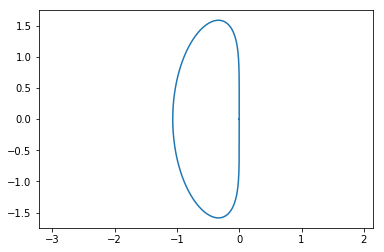
\includegraphics[width=0.5\textwidth]{wenol.png}
  \end{center}
\end{frame}

\begin{frame}{Coefficient d'amplification de WENO}
  Calculs assistés par ordinateur avec \texttt{SymPy} : analyse de von Neumann sur WENO en espérant que ça marche
  
  \begin{center}
    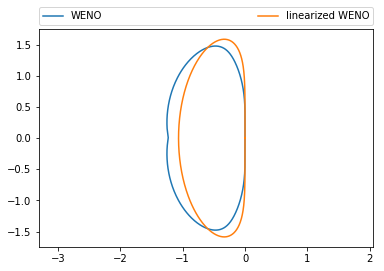
\includegraphics[width=0.5\textwidth]{weno.png}
  \end{center}
\end{frame}


\begin{frame}{Polynôme caractéristique}
  Pour des méthodes type Runge-Kutta explicites :
  \begin{itemize}
    \item Pour une méthode RK($n$,$n$) : troncature du développement de Taylor de l'exponentiel : $$p^{(n,n)}(z) = \sum_{k=0}^n \frac{z^k}{k!}$$
    \item Pour une méthode RK($s$,$n$), $s>n$ : $$p^{(s,n)}(z) = \sum_{k=0}^n \frac{z^k}{k!} + \sum_{k=n+1}^s \alpha_k z^k$$ avec $\alpha_{n+1} \neq \frac{1}{(n+1)!}$
  \end{itemize}
\end{frame}
\begin{frame}{Obtention du polynôme caractéristique}
  Résolution de : $$\dot{u} = L(u)$$
  \begin{enumerate}
    \item Écriture du schéma de la méthode RK à étudier
    \item $L(u) \mapsto \lambda u$
    \item $\lambda\Delta t \mapsto z$
  \end{enumerate}

  Exemple RK(3,3) Shu-Osher: $$
    \begin{aligned}
      u^{(1)} &= u^n + \Delta t L(u^n)                                                & \mapsto & u^{(1)} = u^n + \Delta t \lambda u^n \\
      u^{(2)} &= \frac{3}{4}u^n + \frac{1}{4}u^{(1)} + \frac{1}{4}\Delta t L(u^{(1)}) & \mapsto & u^{(2)} = \frac{3}{4}u^n + \frac{1}{4}u^{(1)} + \frac{1}{4}\Delta t \lambda u^{(1)} \\
      u^{n+1} &= \frac{1}{3}u^n + \frac{2}{3}u^{(2)} + \frac{2}{3}\Delta t L(u^{(2)}) & \mapsto & u^{n+1} = \frac{1}{3}u^n + \frac{2}{3}u^{(2)} + \frac{2}{3}\Delta t \lambda u^{(2)}
    \end{aligned}
  $$

  $$
    u^{n+1} = \underbrace{\left( 1 + z + \frac{z^2}{2} + \frac{z^3}{6} \right)}_{p^{(3,3)}(z)}u^n
  $$
\end{frame}

\begin{frame}{Exemples de domaines de stabilité}
  \begin{center}
    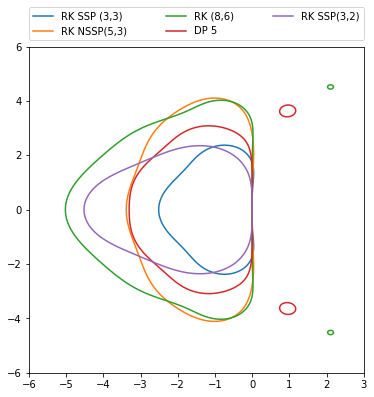
\includegraphics[width=0.5\textwidth]{rk.png}
  \end{center}
\end{frame}

\begin{frame}{Estimation automatique de CFL}
  \begin{enumerate}
    \item Discrétiser $\phi \in [0,2\pi] \equiv [-\pi,\pi]$
    \item Évaluer le coefficient d'amplification sur ces points : $w(\phi)$
    \item Évaluer la frontière du domaine de stabilité $r(\theta)$
    \item $\forall \phi, \rho(\phi) = \argmin_{r(\theta)} (\arg(r(\theta)-w(\phi))) $
    \item $\sigma(\phi) = \left|\frac{\rho(\phi)}{w(\phi)}\right|$
    \item CFL $\sigma = \min_\phi \sigma(\phi)$
  \end{enumerate}
  \begin{center}
    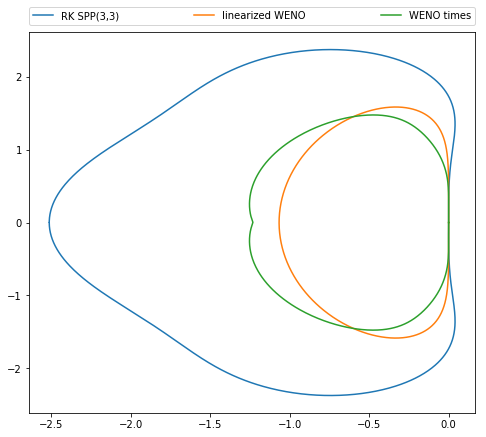
\includegraphics[width=0.4\textwidth]{autocfl.png}
  \end{center}
\end{frame}

\begin{frame}{Quelques CFL}
  \only<1>{
    \begin{center}
      \begin{tabular}{l | c | c | c}
        Méthode RK & étages $s$ & $\sigma$ & Coût par unité de temps $\propto \frac{s}{\sigma}$ \\
        \hline
        WENO$^\ell$-RK(3,3) & 3 & $1.433$ & -- \\
        \hline
        RK SSP(3,3) & 3 & $1.606$ & $1.86$ \\
        RK SSP(4,3) & 4 & $1.923$ & $2.08$ \\
        RK SSP(4,4) & 4 & $1.680$ & $2.38$ \\
        RK (5,3)    & 5 & $2.538$ & $1.97$ \\
        RK (7,6)    & 7 & $1.756$ & $3.99$ \\
        RK (8,6)    & 8 & $2.564$ & $3.12$ \\
      \end{tabular}
    \end{center}
    \begin{center}
      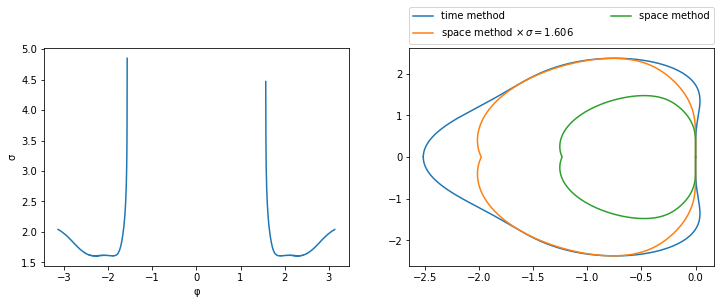
\includegraphics[width=0.7\textwidth]{cfl.png}
    \end{center}
  }
  \only<2>{
    \begin{center}
      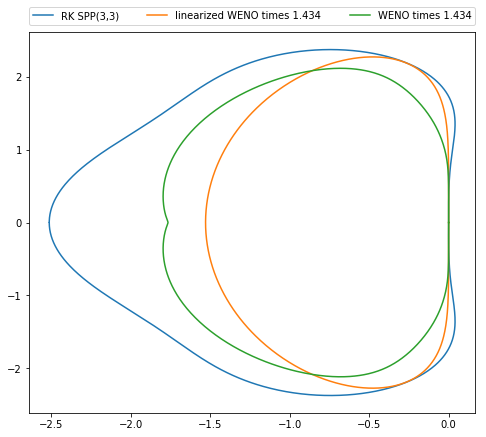
\includegraphics[width=0.7\textwidth]{autocfl1.png}
    \end{center}
  }
  \only<3>{
    \begin{center}
      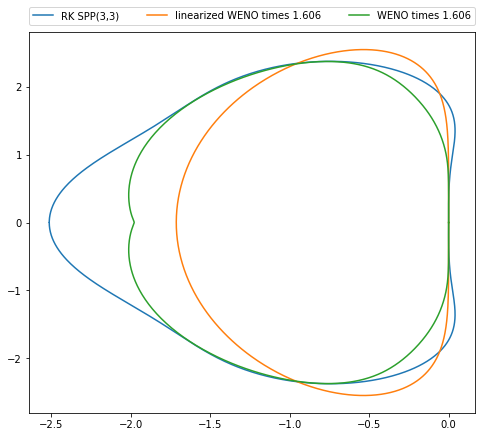
\includegraphics[width=0.7\textwidth]{autocfl2.png}
    \end{center}
  }
\end{frame}

\begin{frame}{Validation de CFL}
  \begin{center}
    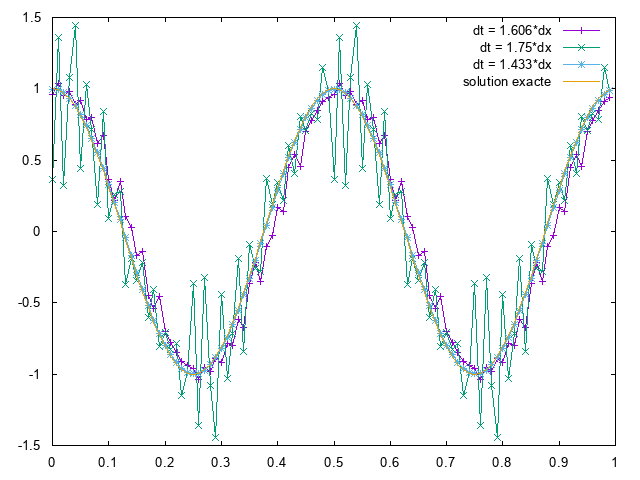
\includegraphics[width=0.85\textwidth]{simuCFL.png}
  \end{center}
\end{frame}

\section{Mise en application dans l'équation de Vlasov}
\begin{frame}{Mise en situation dans l'équation de Vlasov}
  \textbf{Problème :} condition CFL dominée par la vitesse $$\Delta t \leq \sigma\frac{\Delta x}{v_{\text{max}}}\ ,\quad \text{avec } [-v_{\text{max}},v_{\text{max}} ] \equiv \mathbb{R}$$ 
  \begin{itemize}
    \item FFT en $x$ de Vlasov-Poisson : $$\begin{cases}\partial_t \hat{f} + i\kappa v\hat{f} + \widehat{E\partial_vf} = 0 \\ i\kappa \hat{E} = \widehat{\rho - 1} \end{cases}$$
    \item Utilisation de schéma de Lawson (IFRK), écriture exponentielle : $$\begin{cases}\partial_t(e^{i\kappa vt}\hat{f}) + e^{i\kappa vt}\widehat{E\partial_vf} = 0 \\ \hat{E}=-\frac{i}{\kappa}\widehat{\rho-1}\end{cases}$$
    \item WENO uniquement pour approximer $E\partial_v f$, donc CFL : $$\Delta t \leq \sigma \frac{\Delta v}{E_{\text{max}}}$$ avec $E_{\text{max}} \lesssim 0.6$
  \end{itemize}
\end{frame}

\begin{frame}{Schéma de Lawson}
  Résolution de $$\partial_tu + Lu + N(u) = 0$$

  \begin{itemize}
    \item Écriture exponentielle : $$\partial_t(e^{Lt}u) + e^{Lt}N(u) = 0$$
    \item Écriture d'une méthode RK($s$,$n$) sur $$\partial_t v + \tilde{N}(v,t) = 0$$ avec $v = e^{Lt}u$, $\tilde{N}(v,t) = e^{Lt}N(e^{-Lt}v)$
    \item Réécriture en fonction de $u$, $L$ et $N$
  \end{itemize}

  Polynôme caractéristique : $$u^{n+1} = \left(p^{(s,n)}(z)\right)e^{L\Delta t} u^n$$ Si $L\in i\mathbb{R} \Rightarrow$ même stabilité que RK($s$,$n$)
\end{frame}

\begin{frame}{Recherche du meilleur schéma en temps}
  Le modèle de Vlasov-Poisson préserve l'énergie $$H(t) = \int_\Omega\int_{\mathbb{R}} v^2f\,\mathrm{d}v\,\mathrm{d}x + \int_{\Omega}E^2\,\mathrm{d}x$$

  Mesure de l'erreur $\left\|\frac{H(t)-H(0)}{H(0)}\right\|_\infty$ en fonction du coût numérique $\frac{\Delta t}{s}$ pour chaque méthode RK($s$,$n$) étudiée.
\end{frame}

\begin{frame}{Sélection du meilleur schéma en temps}
  \begin{center}
    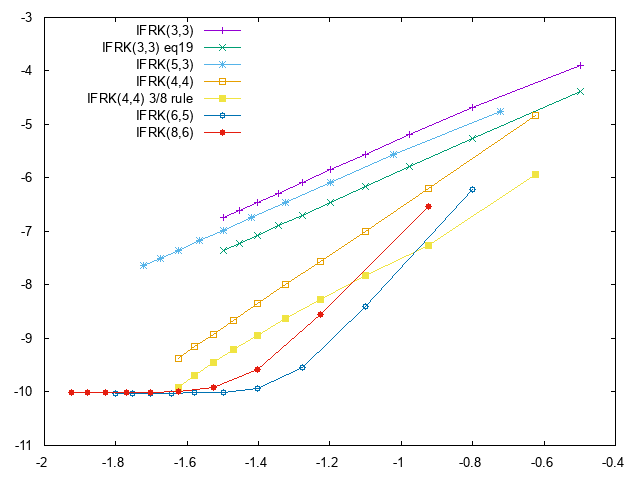
\includegraphics[width=0.85\textwidth]{oHdt.png}
  \end{center}
\end{frame}

\begin{frame}{Conclusion}
  \begin{itemize}
    \item Meilleure estimation du coefficient d'amplification de WENO, en étudiant WENO non linéarisé
    \item Méthode automatique pour évaluer la CFL d'un couple RK($s$,$n$)--WENO5
    \item Schéma spectral en $x$, WENO en $v$, associé au schéma IFRK optimal, avec maximisation de la CFL, validé
  \end{itemize}
\end{frame}

\begin{frame}{Perspectives}
  Maintenant que le code de simulation est validé, on peut tester différentes modélisations
  \begin{itemize}
    \item Implémenter la résolution d'Euler avec un schéma d'ordre élevé
    \item Valider une modélisation hybride fluide-cinétique sur différents profils en vitesse ($\delta_{0}(v) + \mathcal{M}_{\rho_h,u_h,T_h}$) (en lien avec IPP Garching)
    \item Passer à 1D$x$-2D$v$ (Vlasov-Maxwell)
    \item Comprendre un peu mieux pourquoi l'analyse de von Neumann fonctionne sur WENO-JS et pas WENO-M ou WENO-Z
  \end{itemize}
\end{frame}

\begin{frame}{Références}
\nocite{*}
    {\footnotesize
    \bibliographystyle{apalike}
    \bibliography{bib_csi}
    }
\end{frame}

\begin{frame}[t]
  \vfill
  {\usebeamerfont{title}Merci de votre attention}
  \vfill
\end{frame}


\appendix
\backupbegin

\begin{frame}[plain]
  \vspace{0.65\textwidth}
  \hfill\footnotesize{Backup}
\end{frame}

\begin{frame}{Modifications de WENO : WENO-M \& WENO-Z}
  \begin{description}
    \only<1>{
      \item[WENO-JS :] {[G.-S. Jiang \& C.-W. Shu (1996)]} $$\begin{aligned}[t]\alpha_i &\gets \frac{\gamma_i}{(\epsilon + \beta_i)^2} \\ w_i &\gets \frac{\alpha_i}{\sum \alpha_k} \end{aligned}$$ \emph{Paramètre :} $\epsilon = 10^{-6}$
      \item[WENO-M :] {[A. K. Henrick, T. D. Aslam \& J. M. Powers (2005)]} $$\begin{aligned}\alpha_i &\gets \frac{\gamma_i}{(\epsilon + \beta_i)^2} \\ w_i &\gets \frac{\alpha_i}{\sum \alpha_k} \\ g_i &\gets w_i\left(\frac{\gamma_i + \gamma_i^2 - 3w_i\gamma_i + w_i^2}{\gamma_i^2+w_i(1-2\gamma_i)}\right) \\ w_i &\gets \frac{g_i}{\sum g_k} \end{aligned}$$ \emph{Paramètre :} $\epsilon = 10^{-6}$
    }
    \only<2> {
      \item[WENO-Z :] {[R. Borges, M. Carmona, B. Costa \& W. S. Don (2008)]} $$\begin{aligned}\alpha_i &\gets \gamma_i\left(1+\frac{\tau_5}{\epsilon + \beta_i}\right) \\ w_i &\gets \frac{\alpha_i}{\sum \alpha_k} \end{aligned}$$ \emph{Paramètres :} $\epsilon = 10^{-40}$, $\tau_5 = |\beta_0-\beta_2|$
    }
  \end{description}
\end{frame}

\begin{frame}{Modifications de WENO : WENO-M \& WENO-Z}
  \begin{center}
    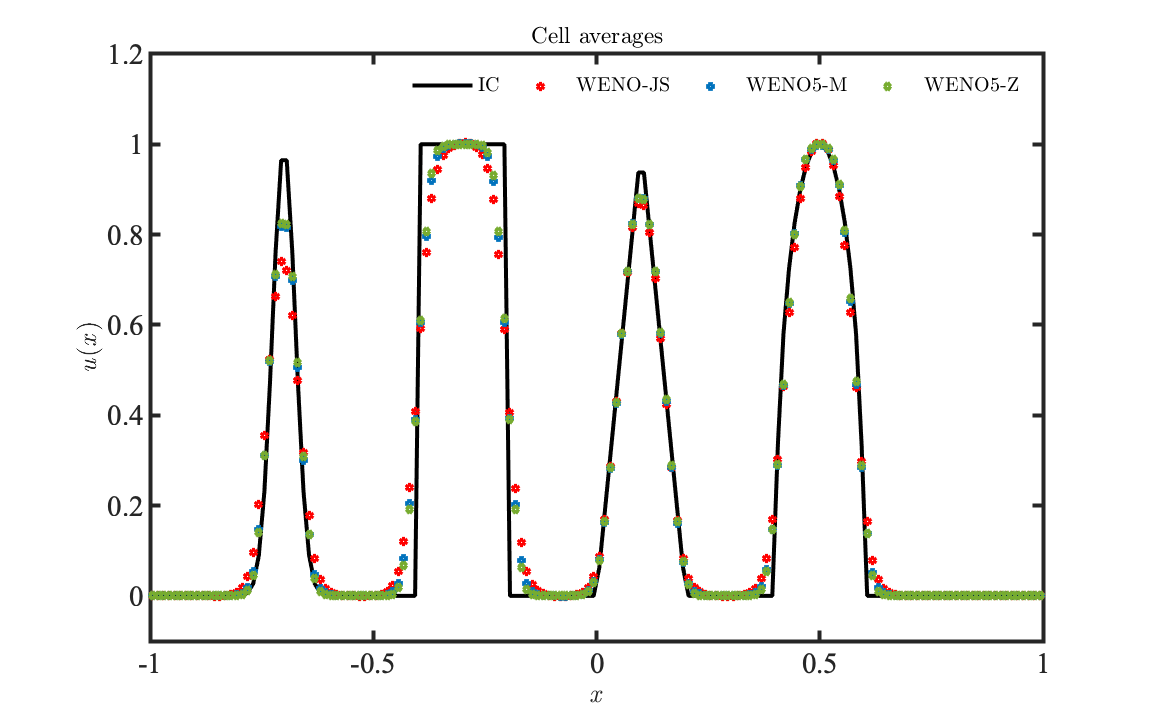
\includegraphics[width=\textwidth]{wenoJSMZ.png}
  \end{center}
\end{frame}

\begin{frame}{WENO$^\ell$}
  \only<1>{
    \textbf{Mesure de l'ordre}
    \begin{center}
      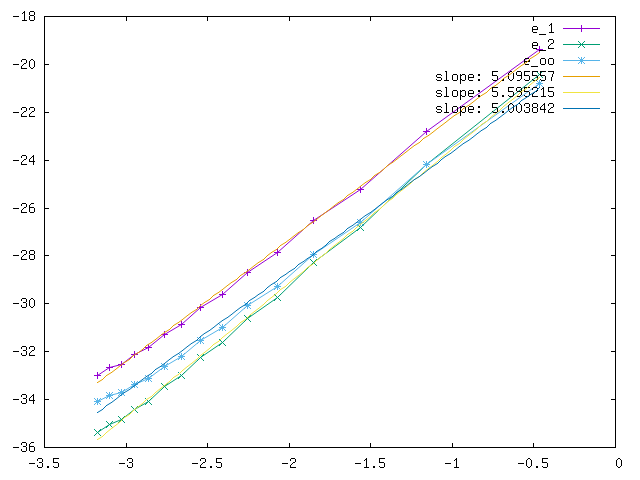
\includegraphics[width=0.85\textwidth]{order_WL.png}
    \end{center}
  }
  \only<2>{
    \textbf{Réaction à une discontinuité}
    \begin{center}
      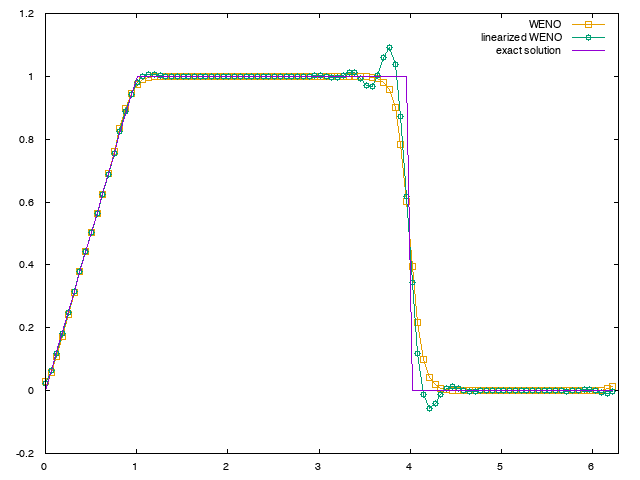
\includegraphics[width=0.85\textwidth]{discontinuity_weno_wenol.png}
    \end{center}
  }
  \only<3>{
    \textbf{Test sur une fonction chapeau}
    \begin{center}
      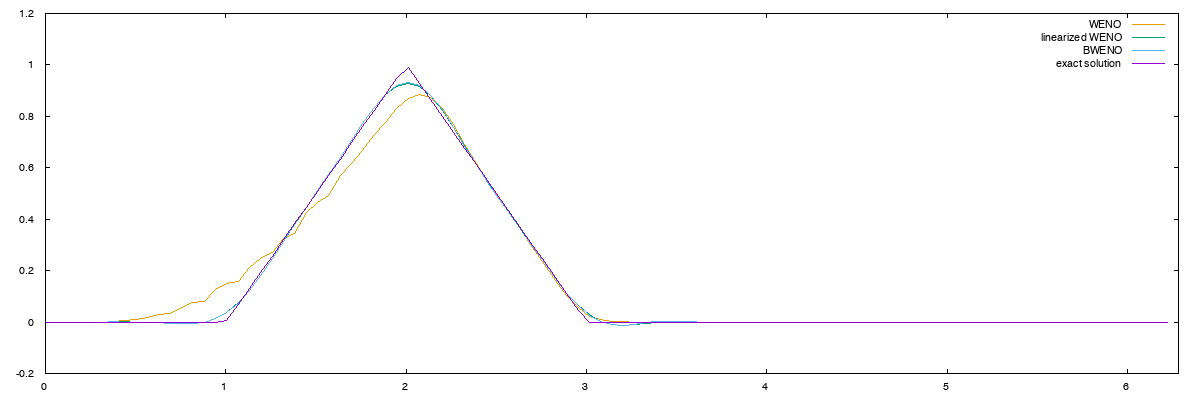
\includegraphics[width=0.80\textwidth]{hat_t2pi_weno_wenol_bweno.png}
      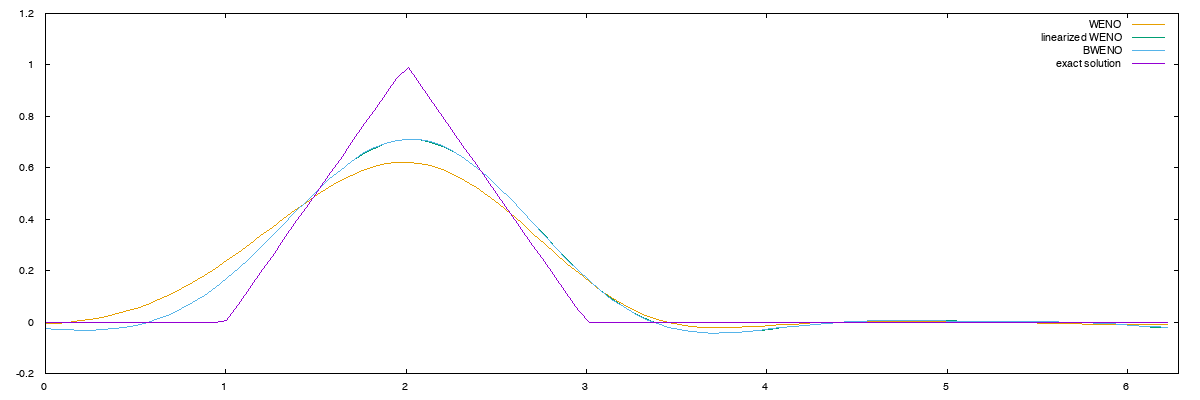
\includegraphics[width=0.80\textwidth]{hat_t300pi_weno_wenol_bweno.png}
    \end{center}
  }
\end{frame}

\backupend

\end{document}